\hypertarget{http-ux534fux8baeux7b80ux4ecb}{%
\subsection{HTTP 协议简介}\label{http-ux534fux8baeux7b80ux4ecb}}

在 Web 应用中,服务器把网页传给浏览器,实际上就是把网页的 HTML
代码发送给浏览器,让浏览器显示出来。而浏览器和服务器之间的传输协议是
HTTP,所以:

\begin{itemize}
\item
  HTML 是一种用来定义网页的文本,会 HTML,就可以编写网页;
\item
  HTTP 是在网络上传输 HTML 的协议,用于浏览器和服务器的通信。
\end{itemize}

在举例子之前,我们需要安装 Google 的
\href{http://www.google.com/intl/zh-CN/chrome/}{Chrome 浏览器}。

为什么要使用 Chrome 浏览器而不是 IE 呢?因为 IE 实在是太慢了,并且,IE
对于开发和调试 Web 应用程序完全是一点用也没有。

我们需要在浏览器很方便地调试我们的 Web 应用,而 Chrome
提供了一套完整地调试工具,非常适合 Web 开发。

安装好 Chrome 浏览器后,打开 Chrome,在菜单中选择
``视图'',``开发者'',``开发者工具'',就可以显示开发者工具:

 
 \begin{figure}[htp]
	\centering
	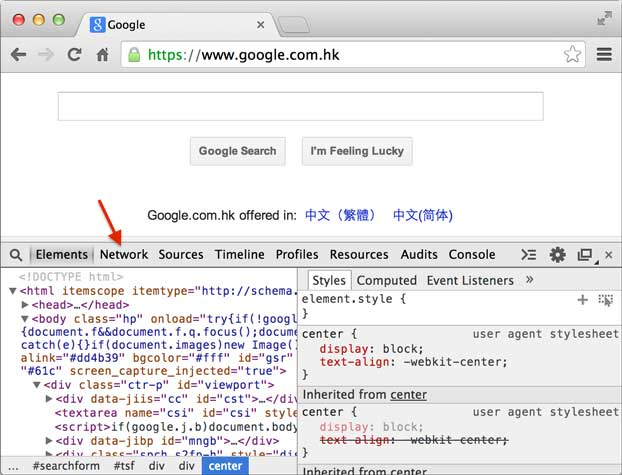
\includegraphics[width=0.6\linewidth]{fig/950415476737952.png}
\end{figure}


\texttt{Elements}显示网页的结构,\texttt{Network}显示浏览器和服务器的通信。我们点\texttt{Network},确保第一个小红灯亮着,Chrome
就会记录所有浏览器和服务器之间的通信:

 
 \begin{figure}[htp]
	\centering
	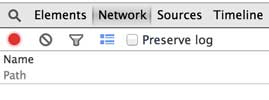
\includegraphics[width=0.6\linewidth]{fig/950415873256992.png}
\end{figure}


当我们在地址栏输入\texttt{www.sina.com.cn}时,浏览器将显示新浪的首页。在这个过程中,浏览器都干了哪些事情呢?通过\texttt{Network}的记录,我们就可以知道。在\texttt{Network}中,定位到第一条记录,点击,右侧将显示\texttt{Request\ Headers},点击右侧的\texttt{view\ source},我们就可以看到浏览器发给新浪服务器的请求:

 
 \begin{figure}[htp]
	\centering
	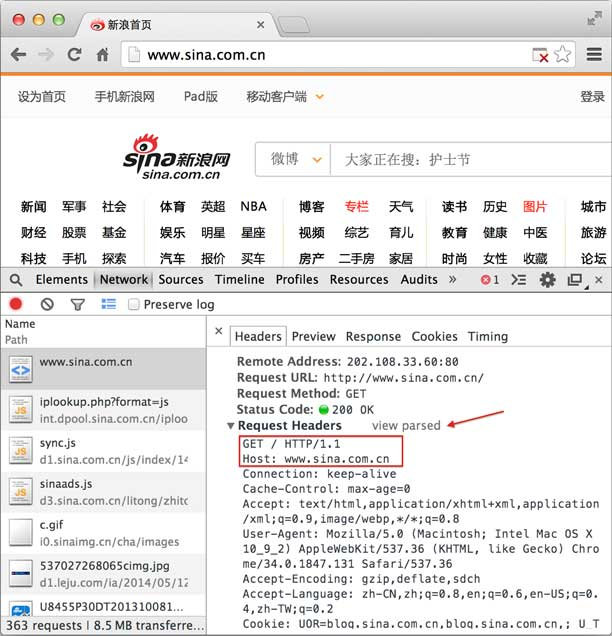
\includegraphics[width=0.6\linewidth]{fig/950413532592512.png}
\end{figure}


最主要的头两行分析如下,第一行:

\begin{pythoncode}
GET / HTTP/1.1
\end{pythoncode}

\texttt{GET}表示一个读取请求,将从服务器获得网页数据,\texttt{/}表示 URL
的路径,URL
总是以\texttt{/}开头,\texttt{/}就表示首页,最后的\texttt{HTTP/1.1}指示采用的
HTTP 协议版本是 1.1。目前 HTTP 协议的版本就是
1.1,但是大部分服务器也支持 1.0 版本,主要区别在于 1.1 版本允许多个 HTTP
请求复用一个 TCP 连接,以加快传输速度。

从第二行开始,每一行都类似于\texttt{Xxx:\ abcdefg}:

\begin{pythoncode}
Host: www.sina.com.cn
\end{pythoncode}

表示请求的域名是\texttt{www.sina.com.cn}。如果一台服务器有多个网站,服务器就需要通过\texttt{Host}来区分浏览器请求的是哪个网站。

继续往下找到\texttt{Response\ Headers},点击\texttt{view\ source},显示服务器返回的原始响应数据:

 
 \begin{figure}[htp]
	\centering
	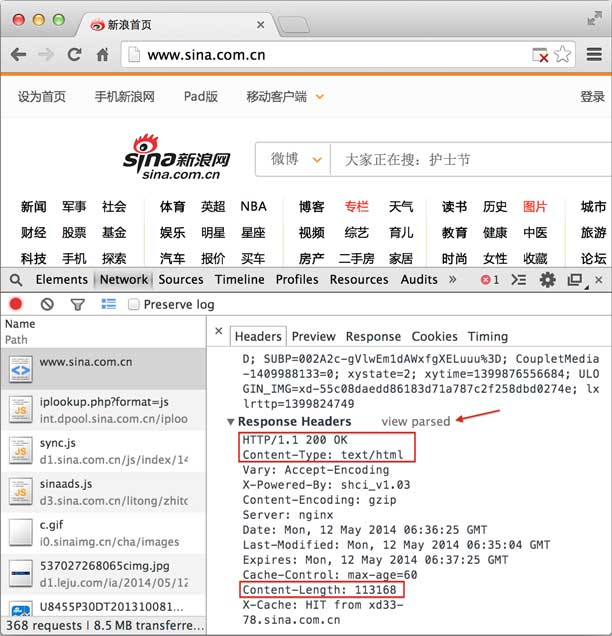
\includegraphics[width=0.6\linewidth]{fig/950413553562752.png}
\end{figure}


HTTP 响应分为 Header 和 Body 两部分(Body
是可选项),我们在\texttt{Network}中看到的 Header 最重要的几行如下:

\begin{pythoncode}
200 OK
\end{pythoncode}

\texttt{200}表示一个成功的响应,后面的\texttt{OK}是说明。失败的响应有\texttt{404\ Not\ Found}:网页不存在,\texttt{500\ Internal\ Server\ Error}:服务器内部出错,等等。

\begin{pythoncode}
Content-Type: text/html
\end{pythoncode}

\texttt{Content-Type}指示响应的内容,这里是\texttt{text/html}表示 HTML
网页。请注意,浏览器就是依靠\texttt{Content-Type}来判断响应的内容是网页还是图片,是视频还是音乐。浏览器并不靠
URL 来判断响应的内容,所以,即使 URL
是\texttt{http://example.com/abc.jpg},它也不一定就是图片。

HTTP 响应的 Body 就是 HTML 源码,我们在菜单栏选择
``视图'',``开发者'',``查看网页源码'' 就可以在浏览器中直接查看 HTML
源码:

 
 \begin{figure}[htp]
	\centering
	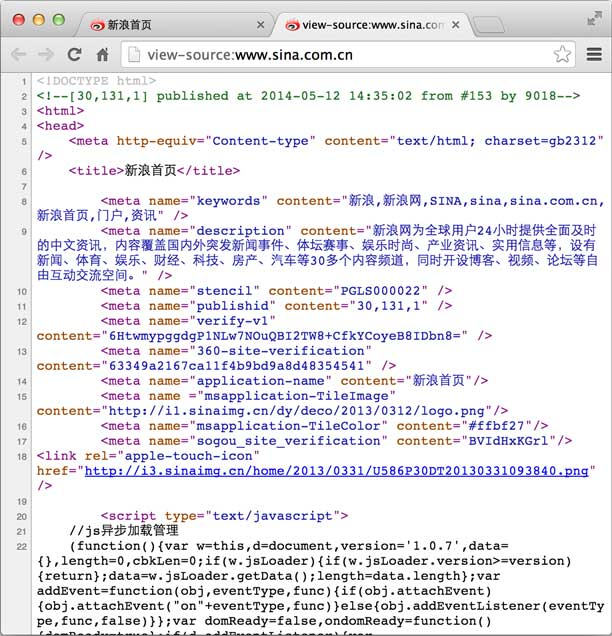
\includegraphics[width=0.6\linewidth]{fig/950413570828960.png}
\end{figure}


当浏览器读取到新浪首页的 HTML 源码后,它会解析
HTML,显示页面,然后,根据 HTML 里面的各种链接,再发送 HTTP
请求给新浪服务器,拿到相应的图片、视频、Flash、JavaScript 脚本、CSS
等各种资源,最终显示出一个完整的页面。所以我们在\texttt{Network}下面能看到很多额外的
HTTP 请求。

\hypertarget{http-ux8bf7ux6c42}{%
\subsubsection{HTTP 请求}\label{http-ux8bf7ux6c42}}

跟踪了新浪的首页,我们来总结一下 HTTP 请求的流程:

步骤 1:浏览器首先向服务器发送 HTTP 请求,请求包括:

方法:\texttt{GET}还是\texttt{POST},\texttt{GET}仅请求资源,\texttt{POST}会附带用户数据;

路径:\texttt{/full/url/path};

域名:由 Host 头指定:\texttt{Host:\ www.sina.com.cn}

以及其他相关的 Header;

如果是 POST,那么请求还包括一个 Body,包含用户数据。

步骤 2:服务器向浏览器返回 HTTP 响应,响应包括:

响应代码:\texttt{200}表示成功,\texttt{3xx}表示重定向,\texttt{4xx}表示客户端发送的请求有错误,\texttt{5xx}表示服务器端处理时发生了错误;

响应类型:由\texttt{Content-Type}指定,例如:\texttt{Content-Type:\ text/html;charset=utf-8}表示响应类型是
HTML
文本,并且编码是\texttt{UTF-8},\texttt{Content-Type:\ image/jpeg}表示响应类型是
JPEG 格式的图片;

以及其他相关的 Header;

通常服务器的 HTTP 响应会携带内容,也就是有一个
Body,包含响应的内容,网页的 HTML 源码就在 Body 中。

步骤 3:如果浏览器还需要继续向服务器请求其他资源,比如图片,就再次发出
HTTP 请求,重复步骤 1、2。

Web 采用的 HTTP 协议采用了非常简单的请求 -
响应模式,从而大大简化了开发。当我们编写一个页面时,我们只需要在 HTTP
响应中把 HTML
发送出去,不需要考虑如何附带图片、视频等,浏览器如果需要请求图片和视频,它会发送另一个
HTTP 请求,因此,一个 HTTP 请求只处理一个资源。

HTTP
协议同时具备极强的扩展性,虽然浏览器请求的是\texttt{http://www.sina.com.cn/}的首页,但是新浪在
HTML
中可以链入其他服务器的资源,比如\texttt{\textless{}img\ src="http://i1.sinaimg.cn/home/2013/1008/U8455P30DT20131008135420.png"\textgreater{}},从而将请求压力分散到各个服务器上,并且,一个站点可以链接到其他站点,无数个站点互相链接起来,就形成了
World Wide Web,简称 ``三达不溜''(WWW)。

\hypertarget{http-ux683cux5f0f}{%
\subsubsection{HTTP 格式}\label{http-ux683cux5f0f}}

每个 HTTP 请求和响应都遵循相同的格式,一个 HTTP 包含 Header 和 Body
两部分,其中 Body 是可选的。

HTTP 协议是一种文本协议,所以,它的格式也非常简单。HTTP GET 请求的格式:

\begin{pythoncode}
GET /path HTTP/1.1
Header1: Value1
Header2: Value2
Header3: Value3
\end{pythoncode}

每个 Header
一行一个,换行符是\texttt{\textbackslash{}r\textbackslash{}n}。

HTTP POST 请求的格式:

\begin{pythoncode}
POST /path HTTP/1.1
Header1: Value1
Header2: Value2
Header3: Value3

body data goes here...
\end{pythoncode}

当遇到连续两个\texttt{\textbackslash{}r\textbackslash{}n}时,Header
部分结束,后面的数据全部是 Body。

HTTP 响应的格式:

\begin{pythoncode}
200 OK
Header1: Value1
Header2: Value2
Header3: Value3

body data goes here...
\end{pythoncode}

HTTP 响应如果包含
body,也是通过\texttt{\textbackslash{}r\textbackslash{}n\textbackslash{}r\textbackslash{}n}来分隔的。请再次注意,Body
的数据类型由\texttt{Content-Type}头来确定,如果是网页,Body
就是文本,如果是图片,Body 就是图片的二进制数据。

当存在\texttt{Content-Encoding}时,Body
数据是被压缩的,最常见的压缩方式是
gzip,所以,看到\texttt{Content-Encoding:\ gzip}时,需要将 Body
数据先解压缩,才能得到真正的数据。压缩的目的在于减少 Body
的大小,加快网络传输。

要详细了解 HTTP 协议,推荐
``\href{http://shop.oreilly.com/product/9781565925090.do}{HTTP: The
Definitive Guide}'' 一书,非常不错,有中文译本:

\href{http://t.cn/R7FguRq}{HTTP 权威指南}

